\documentclass[aspectratio=169,11pt,t]{beamer}

% ============================================================
% Theme and typography
% ============================================================

\usetheme{Madrid}
\usecolortheme{default}
\usefonttheme{professionalfonts}

\setbeamertemplate{navigation symbols}{}
\setbeamertemplate{headline}{}

\setbeamertemplate{footline}{%
  \leavevmode\hbox{%
  \begin{beamercolorbox}[wd=.82\paperwidth,ht=2.5ex,dp=1.0ex,leftskip=.8em]{author in head/foot}
    CSCI 2406 --- Computer Organization \& Architecture (ARM64 / AArch64 Reference)
  \end{beamercolorbox}%
  \begin{beamercolorbox}[wd=.18\paperwidth,ht=2.5ex,dp=1.0ex,rightskip=.8em]{date in head/foot}
    \hfill\insertframenumber/\inserttotalframenumber
  \end{beamercolorbox}}
}

\setbeamersize{
  text margin left=0.65cm,
  text margin right=0.65cm
}

\setbeamerfont{frametitle}{size=\Large, series=\bfseries}
\setbeamerfont{block title}{size=\normalsize, series=\bfseries}
\setbeamertemplate{blocks}[rounded][shadow=false]

% Block vertical padding adjustments
\addtobeamertemplate{block begin}{\vspace{0.1em}}{\vspace{0.1em}}
\addtobeamertemplate{block end}{}{\vspace{0.2em}}

% Base list item separation
\setbeamertemplate{itemize/enumerate body begin}{\setlength{\itemsep}{4pt}}
\setbeamertemplate{itemize/enumerate subbody begin}{\setlength{\itemsep}{2pt}}

% ============================================================
% Packages
% ============================================================

\usepackage[T1]{fontenc}
\usepackage{lmodern}
\usepackage{amsmath}
\usepackage{booktabs}
\usepackage{array}
\usepackage{colortbl}
\usepackage{tikz}

\usetikzlibrary{
  arrows.meta,
  positioning,
  shapes.geometric,
  calc,
  decorations.pathreplacing
}

% ============================================================
% Colors
% ============================================================

\definecolor{navy}{RGB}{24,43,68}
\definecolor{deepblue}{RGB}{45,88,130}
\definecolor{lightblue}{RGB}{235,242,250}
\definecolor{softgray}{RGB}{245,247,250}
\definecolor{darkgray}{RGB}{25,28,32}
\definecolor{gold}{RGB}{200,145,35}

\setbeamercolor{palette primary}{bg=navy,fg=white}
\setbeamercolor{palette secondary}{bg=deepblue,fg=white}
\setbeamercolor{frametitle}{bg=navy,fg=white}
\setbeamercolor{title}{fg=white}
\setbeamercolor{subtitle}{fg=white}
\setbeamercolor{author}{fg=white}
\setbeamercolor{date}{fg=white}
\setbeamercolor{titlelike}{fg=white}
\setbeamercolor{block title}{bg=deepblue,fg=white}
\setbeamercolor{block body}{bg=lightblue,fg=darkgray}
\setbeamercolor{normal text}{fg=darkgray,bg=white}

% ============================================================
% Formatting shortcuts
% ============================================================

\setlength{\parskip}{0pt}

\newcommand{\key}[1]{\textbf{#1}}
\newcommand{\bits}[1]{\texttt{#1}}
\newcommand{\hex}[1]{\texttt{0x#1}}
\newcommand{\code}[1]{\texttt{#1}}

% Section divider macro
\newcommand{\sectiondivider}[2]{%
\begin{frame}[plain]
\begin{tikzpicture}[remember picture,overlay]
\fill[navy] (current page.south west) rectangle (current page.north east);
\fill[gold] (current page.south west) rectangle ([yshift=.15cm]current page.south east);
\end{tikzpicture}
\vspace{1.5cm}
\begin{minipage}{0.85\textwidth}
{\color{gold}\large\bfseries #1\par}
\vspace{0.3cm}
{\color{white}\fontsize{22}{26}\selectfont\bfseries #2\par}
\end{minipage}
\end{frame}
}

% ============================================================
% Metadata
% ============================================================

\title[Topic 3]{
  Machine-Level Data Representation
}

\subtitle{
  Binary and hexadecimal representation, signed and unsigned integers,\\
  two's complement representation, and endianness in AArch64
}

\author{
  Computer Organization \& Architecture
}

\date{Topic 3}

% ============================================================
% Presentation Body (36 Frames Total)
% ============================================================

\begin{document}

% --- Slide 1: Title Slide ---
\begin{frame}[plain]
\begin{tikzpicture}[remember picture,overlay]
\fill[navy] (current page.south west) rectangle (current page.north east);
\fill[gold] (current page.south west) rectangle ([yshift=.18cm]current page.south east);
\end{tikzpicture}
\vspace{1.0cm}
\begin{minipage}{0.9\textwidth}
{\color{gold}\large\bfseries CSCI 2406: Topic 03\par}
\vspace{0.3cm}
{\color{white}\fontsize{20}{24}\selectfont\bfseries Machine-Level Data Representation\par}
\vspace{0.3cm}
{\color{lightblue}\normalsize Binary/Hex representation, signed vs unsigned, two's complement, and memory endianness / alignment in AArch64\par}
\vspace{0.6cm}
{\color{softgray}\small Computer Organization \& Architecture \quad\textbar\quad Topic 3\par}
\end{minipage}
\end{frame}

% --- Slide 2: Topic Outline ---
\begin{frame}{Topic 3 Outline}
    \begin{block}{Topic Objective}
        Analysis of how machine-level information is encoded, interpreted, and organized across fixed-width registers and byte-addressed memory structures.
    \end{block}
    \vspace{0.4em}
    \begin{itemize}
        \item \key{Section 1}: Bits, Bytes, Words, and Base Conversions
        \item \key{Section 2}: Binary and Hexadecimal Representation
        \item \key{Section 3}: Unsigned and Signed Integer Representations
        \item \key{Section 4}: Two's Complement Encoding and Arithmetic Behavior
        \item \key{Section 5}: Memory Endianness and Data Alignment in AArch64
        \item \key{Section 6}: Summary and Worked Self-Test Exercises
    \end{itemize}
\end{frame}

% ============================================================
% SECTION 1
% ============================================================
\sectiondivider{Section 01}{Bits, Bytes, Words, and\\Base Conversions}

% --- Slide 4: Why Data Representation Matters ---
\begin{frame}{Why Data Representation Matters}
    All machine-level information is stored as fixed-width bit patterns:
    \vspace{0.2em}
    \begin{itemize}
        \item \key{Context Dependent}: The same bit pattern can mean different things under different interpretations (e.g., \hex{0xFF} can be $255$ unsigned or $-1$ signed).
        \item \key{ISA Rules}: Software interpretation determines whether bits represent data items, memory addresses, or machine instructions.
        \item \key{Fixed-Width Bounds}: Registers impose strict hardware width limits on numeric ranges.
        \item \key{Layout Rules}: Memory organization dictates how multi-byte values are mapped and retrieved.
    \end{itemize}
\end{frame}

% --- Slide 5: Bits, Bytes, and Words ---
\begin{frame}{Data Units in Memory and Registers}
    \begin{block}{Hierarchical Units of Storage}
        \begin{itemize}
            \item \key{Bit}: A single binary digit ($0$ or $1$).
            \item \key{Byte}: Contains $8$ bits; the foundational unit of addressable memory.
            \item \key{Halfword}: Commonly $16$ bits ($2$ bytes).
            \item \key{Word}: Commonly $32$ bits ($4$ bytes) in standard architectures.
            \item \key{Doubleword}: Commonly $64$ bits ($8$ bytes), native to AArch64 registers (\code{x0}--\code{x30}).
        \end{itemize}
    \end{block}
    \vspace{0.2em}
    \begin{block}{Example}
        One AArch64 register width = $64$ bits = $8$ bytes.
    \end{block}
\end{frame}

% --- Slide 6: Binary Number System ---
\begin{frame}{The Binary Number System (Base 2)}
    Binary maps directly to physical dual-state digital hardware:
    \vspace{0.2em}
    \begin{itemize}
        \item Each digit position represents a distinct power of two.
        \item \key{LSB (Least Significant Bit)}: The rightmost bit position ($2^0$).
        \item \key{MSB (Most Significant Bit)}: The leftmost bit position in a fixed-width container.
    \end{itemize}
    \vspace{0.3em}
    \begin{block}{Positional Evaluation Example}
        $$\text{1011}_2 = (1 \times 8) + (0 \times 4) + (1 \times 2) + (1 \times 1) = 8 + 0 + 2 + 1 = 11_{10}$$
    \end{block}
\end{frame}

% --- Slide 7: Converting Binary and Decimal ---
\begin{frame}{Base Conversion Mechanics}
    \begin{columns}[T]
        \begin{column}{0.48\textwidth}
            \begin{block}{Binary to Decimal}
                \begin{itemize}
                    \item Write power-of-two weights above each bit ($2^0, 2^1, 2^2 \dots$).
                    \item Disregard positions where the bit is $0$.
                    \item Sum the weights where the bit is $1$.
                    \item Example: $01010110_2 = 64 + 16 + 4 + 2 = 86_{10}$.
                \end{itemize}
            \end{block}
        \end{column}
        \begin{column}{0.48\textwidth}
            \begin{block}{Decimal to Binary}
                \begin{itemize}
                    \item Repeatedly divide the decimal value by $2$.
                    \item Record each remainder as a binary digit.
                    \item Read remainders from bottom to top.
                    \item Pad with leading zeros to match container width.
                    \item Example: $13_{10} = 1101_2$.
                \end{itemize}
            \end{block}
        \end{column}
    \end{columns}
\end{frame}

% ============================================================
% SECTION 2
% ============================================================
\sectiondivider{Section 02}{Binary and Hexadecimal Representation}

% --- Slide 9: Hexadecimal Number System ---
\begin{frame}{The Hexadecimal Number System (Base 16)}
    Hexadecimal provides a compact, readable shorthand for machine-level data:
    \vspace{0.2em}
    \begin{itemize}
        \item Digits range from $0$ to $9$ and letters $A$ to $F$ (representing values $10$ to $15$).
        \item \key{Exact Mapping}: Each single hexadecimal digit maps precisely to $4$ binary bits ($2^4 = 16$).
        \item Used universally for memory addresses, instruction opcodes, and register dumps.
    \end{itemize}
    \vspace{0.3em}
    \begin{block}{Example}
        $$\text{0x2A} = 0010\,1010_2 = (2 \times 16) + 10 = 42_{10}$$
    \end{block}
\end{frame}

% --- Slide 10: Binary-Hexadecimal Conversion ---
\begin{frame}{Direct Binary-Hexadecimal Conversion}
    Converting between binary and hex requires no intermediate decimal math:
    \vspace{0.3em}
    \begin{columns}[T]
        \begin{column}{0.48\textwidth}
            \begin{block}{Binary to Hexadecimal}
                \begin{itemize}
                    \item Group binary bits into sets of four starting from the right (LSB).
                    \item Pad the leftmost group with leading zeros if necessary.
                    \item Map each 4-bit nibble directly to its hex digit.
                    \item Example: $1101\,0110_2 = \text{0xD6}$.
                \end{itemize}
            \end{block}
        \end{column}
        \begin{column}{0.48\textwidth}
            \begin{block}{Hexadecimal to Binary}
                \begin{itemize}
                    \item Take each individual hex character.
                    \item Expand it into its exact 4-bit binary equivalent.
                    \item Concatenate the nibbles together.
                    \item Example: $\text{0x5F} = 0101\,1111_2$.
                \end{itemize}
            \end{block}
        \end{column}
    \end{columns}
\end{frame}

% --- Slide 11: AArch64 Registers and Data Widths ---
\begin{frame}{AArch64 Registers and Data Widths}
    AArch64 general-purpose registers are 64 bits wide, supporting flexible data sizing:
    \vspace{0.2em}
    \begin{itemize}
        \item A 64-bit register (\code{x0}--\code{x30}) holds $64$ bits of raw data bits.
        \item The exact same bit pattern can be interpreted as signed integers, unsigned integers, pointers, or masks.
        \item Memory instructions (\code{ldr}, \code{str}) explicitly specify access sizes (bytes, halfwords, words, doublewords).
    \end{itemize}
    \vspace{0.3em}
    \begin{block}{Example Interpretation}
        Setting \code{x0 = 0xFFFFFFFFFFFFFFFF} can represent the unsigned integer $18,446,744,073,709,551,615$ or the signed integer $-1$.
    \end{block}
\end{frame}

% ============================================================
% SECTION 3
% ============================================================
\sectiondivider{Section 03}{Unsigned and Signed Integer Representations}

% --- Slide 13: Unsigned Integer Representation ---
\begin{frame}{Unsigned Integer Representation}
    Unsigned integers represent only non-negative values ($0$ and positive integers):
    \vspace{0.2em}
    \begin{itemize}
        \item Every bit position contributes a strictly positive power-of-two weight.
        \item The leftmost bit (MSB) acts as a high-order magnitude bit, not a sign indicator.
        \item An $n$-bit unsigned container spans the exact range from $0$ to $2^n - 1$.
    \end{itemize}
    \vspace{0.3em}
    \begin{block}{Unsigned Range Examples}
        \begin{itemize}
            \item 8-bit unsigned range: $0$ to $2^8 - 1 = 255$.
            \item 64-bit unsigned range: $0$ to $2^{64} - 1 \approx 1.84 \times 10^{19}$.
            \item Example: $1111\,1111_2 = 255$ (in 8 bits).
        \end{itemize}
    \end{block}
\end{frame}

% --- Slide 14: Unsigned Arithmetic Overflow ---
\begin{frame}{Unsigned Arithmetic and Fixed-Width Limits}
    Unsigned operations are evaluated modulo $2^n$ for an $n$-bit container:
    \vspace{0.2em}
    \begin{itemize}
        \item \key{Fixed-Width Bound}: When an unsigned addition or operation exceeds the maximum representable value ($2^n - 1$), the fixed-width register cannot expand.
        \item \key{Truncation \& Modular Behavior}: High-order carry bits exceeding the bit-width are truncated, leaving the remainder value constrained to the modular range modulo ${2^n}$.
        \item Processors record unsigned carry-out conditions in status flags.
    \end{itemize}
    \vspace{0.3em}
    \begin{block}{Classic Overflow Example}
        In 8-bit unsigned arithmetic:
        $$255 + 1 = 1111\,1111_2 + 1 = 0000\,0000_2 = 0 \quad (\text{with Carry Out})$$
    \end{block}
\end{frame}

% --- Slide 15: Signed Integer Representation & Sign-Magnitude Flaws ---
\begin{frame}{Signed Integer Challenges \& Sign-Magnitude Failure}
    Signed integers require encoding both positive and negative values:
    \vspace{0.2em}
    \begin{itemize}
        \item \key{Naïve Approach (Sign-Magnitude)}: Dedicate the MSB as a sign flag ($0 = \text{positive}, 1 = \text{negative}$).
        \item \key{Fatal Flaws of Sign-Magnitude}:
        \begin{itemize}
            \item \textbf{Dual Zeros}: Encodes both positive zero ($00000$) and negative zero ($10000$).
            \item \textbf{Broken Arithmetic}: Standard hardware adders fail when adding positive and negative numbers (e.g., $+3 + (-3) \rightarrow 00011 + 10011 = 10110 (-6)$, which is incorrect).
        \end{itemize}
    \end{itemize}
    \vspace{0.2em}
    \begin{block}{The Engineering Solution}
        Modern computer systems bypass these hardware flaws by adopting \key{two's complement representation}.
    \end{block}
\end{frame}

% ============================================================
% SECTION 4
% ============================================================
\sectiondivider{Section 04}{Two's Complement Representation\\and Arithmetic Behavior}

% --- Slide 17: Two's Complement Solution ---
\begin{frame}{Two's Complement Representation}
    \begin{block}{Core Design Objectives}
        Two's complement provides a robust signed number system requiring \key{no special additional hardware} for add, subtract, or multiply units, while maintaining a single unique zero.
    \end{block}
    \vspace{0.3em}
    \begin{block}{Algorithm for Negation (Forming Two's Complement)}
        \begin{enumerate}
            \item Start with the positive magnitude in binary.
            \item \key{Invert every bit} ($0 \rightarrow 1, 1 \rightarrow 0$) to produce the one's complement.
            \item \key{Add 1} to the inverted result to produce the final two's complement encoding.
        \end{enumerate}
    \end{block}
    \vspace{0.2em}
    \begin{itemize}
        \item Example (-5 in 8 bits): $+5 = 0000\,0101 \rightarrow \text{invert} = 1111\,1010 \rightarrow \text{add } 1 = 1111\,1011$.
    \end{itemize}
\end{frame}

% --- Slide 18: Two's Complement Adder Execution ---
\begin{frame}{Two's Complement in Action: $-9 + 6$}
    Standard hardware adders evaluate signed numbers correctly without modification:
    \vspace{0.2em}
    \begin{center}
        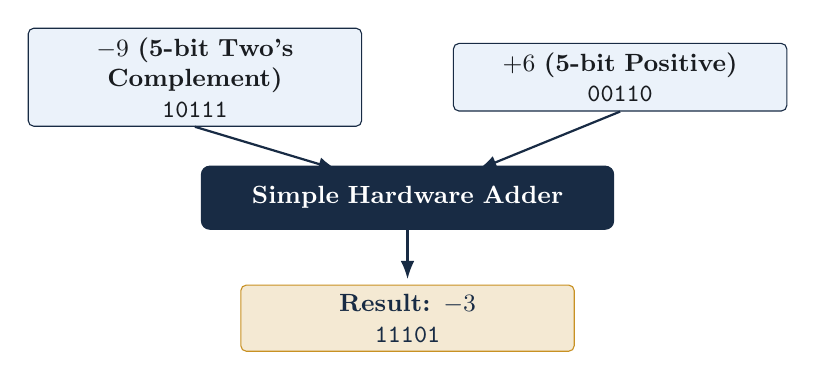
\begin{tikzpicture}[scale=0.9, every node/.style={font=\small}]
            % Input boxes (top boxes centered at y = 2.4, height spans roughly from y = 2.0 to 2.8)
            \node[draw=navy, fill=lightblue, text=darkgray, rounded corners=2pt, text width=4.0cm, align=center] (b1) at (0,2.4) {
                \textbf{$-9$ (5-bit Two's Complement)}\\
                \code{10111}
            };
            \node[draw=navy, fill=lightblue, text=darkgray, rounded corners=2pt, text width=4.0cm, align=center] (b2) at (6.0,2.4) {
                \textbf{$+6$ (5-bit Positive)}\\
                \code{00110}
            };
            
            % Adder box
            \node[draw=navy, fill=navy, text=white, rounded corners=3pt, text width=5.0cm, align=center, minimum height=0.8cm] (adder) at (3.0,0.7) {
                \textbf{Simple Hardware Adder}
            };
            
            % Output box
            \node[draw=gold, fill=gold!20, text=navy, rounded corners=2pt, text width=4.0cm, align=center] (out) at (3.0,-1.0) {
                \textbf{Result: $-3$}\\
                \code{11101}
            };
            
            % Arrows starting precisely from the bottom borders of the input boxes down to the adder
            \draw[thick, -Latex, draw=navy] (b1.south) -- (2.0,1.1);
            \draw[thick, -Latex, draw=navy] (b2.south) -- (4.0,1.1);
            \draw[thick, -Latex, draw=navy] (3.0,0.3) -- (3.0,-0.45);
        \end{tikzpicture}
    \end{center}
    \vspace{-0.1em}
    \begin{itemize}
        \item Adding \code{10111} ($-9$) and \code{00110} ($+6$) yields \code{11101} (which evaluates exactly to $-3$).
    \end{itemize}
\end{frame}

% --- Slide 19: Two's Complement Range ---
\begin{frame}{Two's Complement Numeric Range}
    An $n$-bit container under two's complement encoding spans asymmetric bounds:
    \vspace{0.2em}
    \begin{itemize}
        \item \key{Total Patterns}: $2^n$ unique bit combinations.
        \item \key{Signed Range}: $-2^{n-1}$ to $2^{n-1} - 1$.
        \item \key{Asymmetry}: There is always \textbf{one more negative value} than positive value because zero consumes one positive pattern.
        \item The most negative value has only its sign bit set ($1000\dots 0$).
    \end{itemize}
    \vspace{0.3em}
    \begin{block}{8-Bit and 64-Bit Ranges}
        \begin{itemize}
            \item 8-bit two's complement range: $-128$ to $+127$.
            \item 64-bit two's complement range: $-9,223,372,036,854,775,808$ to $+9,223,372,036,854,775,807$.
        \end{itemize}
    \end{block}
\end{frame}

% --- Slide 20: Signed Overflow Detection ---
\begin{frame}{Signed Arithmetic Overflow}
    \begin{block}{Definition of Signed Overflow}
        Signed overflow occurs when the true mathematical result of an operation falls outside the representable signed range of the destination container.
    \end{block}
    \vspace{0.3em}
    \begin{itemize}
        \item \key{Symptom}: Adding two positive numbers yields a negative result, or adding two negative numbers yields a positive result.
        \item \key{Detection}: Hardware cannot detect overflow merely by looking at the final bit pattern; it evaluates carry inputs and outputs into the MSB.
        \item \key{Status Flags}: AArch32/AArch64 condition flags record signed overflow in the \key{V} (Overflow) flag.
        \item Example: In 8-bit math, $127 + 1 = 0111\,1111 + 0000\,0001 = 1000\,0000 (-128)$, triggering an immediate overflow exception/flag.
    \end{itemize}
\end{frame}

% ============================================================
% SECTION 5
% ============================================================
\sectiondivider{Section 05}{Memory Endianness and\\Data Alignment in AArch64}

% --- Slide 22: Memory as a Byte-Addressed Structure ---
\begin{frame}{Memory as a Byte-Addressed Structure}
    AArch64 memory is organized as a linear array of individually addressable bytes:
    \vspace{0.2em}
    \begin{itemize}
        \item Each unique memory address references exactly one $8$-bit byte.
        \item Multi-byte data structures (halfwords, words, doublewords) occupy consecutive sequential byte addresses.
        \item \key{Address Pointer}: A 64-bit multi-byte value is identified by the address of its lowest-numbered byte container.
    \end{itemize}
    \vspace{0.3em}
    \begin{block}{Example: 64-Bit Doubleword Layout}
        A 64-bit doubleword stored at pointer address \hex{0x1000} occupies physical byte addresses \hex{0x1000}, \hex{0x1001}, \hex{0x1002}, \hex{0x1003}, \hex{0x1004}, \hex{0x1005}, \hex{0x1006}, and \hex{0x1007}.
    \end{block}
\end{frame}

% --- Slide 23: Endianness Definition ---
\begin{frame}{Endianness: Ordering Multi-Byte Values}
    \begin{block}{Definition}
        \key{Endianness} defines the sequential byte ordering used when storing multi-byte values across consecutive memory addresses.
    \end{block}
    \vspace{0.3em}
    \begin{columns}[T]
        \begin{column}{0.48\textwidth}
            \begin{block}{Big-Endian Ordering}
                \begin{itemize}
                    \item Stores the \key{most significant byte (MSB)} at the lowest memory address.
                    \item Matches reading human numerical text (left-to-right).
                \end{itemize}
            \end{block}
        \end{column}
        \begin{column}{0.48\textwidth}
            \begin{block}{Little-Endian Ordering}
                \begin{itemize}
                    \item Stores the \key{least significant byte (LSB)} at the lowest memory address.
                    \item Standard default layout for modern ARM64 and x86 architectures.
                \end{itemize}
            \end{block}
        \end{column}
    \end{columns}
\end{frame}

% --- Slide 24: Endianness in AArch64 ---
\begin{frame}{Little-Endian Layout in AArch64 Practice}
    AArch64 systems default to little-endian memory organization:
    \vspace{0.2em}
    \begin{itemize}
        \item The underlying numeric value held in a register remains unaffected by byte layout.
        \item Load instructions reconstruct registers from memory bytes; store instructions decompose register values into byte streams.
        \item Endianness becomes explicitly visible when inspecting raw memory byte dumps.
    \end{itemize}
    \vspace{0.3em}
    \begin{block}{Concrete Layout Example}
        Storing 64-bit value \hex{0x1234567890ABCDEF} at address \hex{0x2000} in little-endian order places bytes in ascending memory addresses as:
        $$\text{\hex{EF}}\ (\text{at } \hex{2000}),\ \text{\hex{CD}},\ \text{\hex{AB}},\ \text{\hex{90}},\ \text{\hex{78}},\ \text{\hex{56}},\ \text{\hex{34}},\ \text{\hex{12}}\ (\text{at } \hex{2007})$$
    \end{block}
\end{frame}

% --- Slide 25: Data Alignment in AArch64 ---
\begin{frame}{Data Alignment in AArch64}
    \begin{block}{Definition of Natural Alignment}
        Data alignment requires that a variable of size $n$ bytes be stored at a memory address that is an exact multiple of $n$.
    \end{block}
    \vspace{0.3em}
    \begin{itemize}
        \item \key{64-Bit Doubleword}: Naturally aligned at addresses divisible by $8$ ($0, 8, 16 \dots$).
        \item \key{32-Bit Word}: Naturally aligned at addresses divisible by $4$.
        \item \key{16-Bit Halfword}: Naturally aligned at addresses divisible by $2$.
        \item \key{Hardware Efficiency}: Aligned memory transactions execute with maximum speed and single-cycle bus efficiency.
        \item Misaligned accesses can trigger hardware traps, alignment faults, or severe performance penalties.
    \end{itemize}
\end{frame}

% ============================================================
% SECTION 6
% ============================================================
\sectiondivider{Section 06}{Summary \& Self-Test}

% --- Slide 27: Topic Summary ---
\begin{frame}{Topic 3 Comprehensive Summary}
    \begin{itemize}
        \item \key{Fixed-Width Representation}: Information is stored as bit patterns whose semantics depend entirely on software and ISA interpretation.
        \item \key{Base Conversions}: Binary ($Base\ 2$) and Hexadecimal ($Base\ 16$) provide readable notations for digital machine states.
        \item \key{Unsigned Integers}: Represent non-negative values with strict upper limits and modulo truncation upon overflow.
        \item \key{Two's Complement}: The industry standard for signed integers, enabling negative values without special ALU hardware.
        \item \key{Endianness \& Alignment}: AArch64 utilizes little-endian byte ordering and strict natural data alignment for memory access performance.
    \end{itemize}
\end{frame}

% --- Slide 28: Self-Test: Questions 1 & 2 ---
\begin{frame}{Self-Test: Questions 1 \& 2}
    \begin{block}{Question 1: Bits, Words, and Bases}
        What is the relationship between bits, bytes, words, and 64-bit AArch64 registers? Why is hexadecimal universally preferred over binary when inspecting memory dumps?
    \end{block}
    \vspace{0.4em}
    \begin{block}{Question 2: Unsigned Arithmetic Limits}
        What range of values can be represented by an unsigned $n$-bit integer? What happens when an 8-bit unsigned accumulator holding $255$ has $1$ added to it?
    \end{block}
\end{frame}

% --- Slide 29: Self-Test: Solutions 1 & 2 ---
\begin{frame}{Self-Test: Solutions 1 \& 2}
    \begin{block}{Solution 1}
        Bits are binary digits; 8 bits make a byte; words are 32 bits; AArch64 general-purpose registers are 64 bits (doublewords) wide. Hexadecimal is compact, mapping each single character directly to a 4-bit nibble without conversion fuzziness.
    \end{block}
    \vspace{0.3em}
    \begin{block}{Solution 2}
        An unsigned $n$-bit container spans $0$ to $2^n - 1$. Adding $1$ to $255$ in an 8-bit container exceeds the fixed-width capacity, resulting in truncation modulo $2^8$, producing $0$ and setting the carry flag.
    \end{block}
\end{frame}

% --- Slide 30: Self-Test: Questions 3 & 4 ---
\begin{frame}{Self-Test: Questions 3 \& 4}
    \begin{block}{Question 3: Two's Complement Negation}
        How do you form the two's complement negative of a positive binary number? What signed range is representable in a 32-bit two's complement integer container?
    \end{block}
    \vspace{0.4em}
    \begin{block}{Question 4: Signed vs. Unsigned Interpretation}
        How can the exact same 32-bit bit pattern represent two completely different values when interpreted as signed versus unsigned?
    \end{block}
\end{frame}

% --- Slide 31: Self-Test: Solutions 3 & 4 ---
\begin{frame}{Self-Test: Solutions 3 \& 4}
    \begin{block}{Solution 3}
        To form a two's complement negative, take the binary magnitude, invert every bit (one's complement), and add $1$. A 32-bit two's complement container spans $-2^{31}$ to $2^{31} - 1$ ($-2,147,483,648$ to $+2,147,483,647$).
    \end{block}
    \vspace{0.3em}
    \begin{block}{Solution 4}
        Unsigned interpretation treats all bits as positive power-of-two weights. Signed two's complement interpretation assigns the MSB a negative weight. Thus, \hex{0xFFFFFFFF} equals $4,294,967,295$ unsigned but $-1$ signed.
    \end{block}
\end{frame}

% --- Slide 32: Self-Test: Questions 5 & 6 ---
\begin{frame}{Self-Test: Questions 5 \& 6}
    \begin{block}{Question 5: Endianness in Memory}
        What is the fundamental difference between little-endian and big-endian byte ordering? Which convention does AArch64 use by default?
    \end{block}
    \vspace{0.4em}
    \begin{block}{Question 6: Data Alignment}
        What does data alignment mean in computer architecture, and why are naturally aligned memory addresses important for performance?
    \end{block}
\end{frame}

% --- Slide 33: Self-Test: Solutions 5 & 6 ---
\begin{frame}{Self-Test: Solutions 5 \& 6}
    \begin{block}{Solution 5}
        Little-endian stores the least significant byte (LSB) at the lowest memory address, whereas big-endian stores the most significant byte (MSB) at the lowest address. AArch64 uses little-endian byte ordering by default.
    \end{block}
    \vspace{0.3em}
    \begin{block}{Solution 6}
        Data alignment requires variables of size $n$ to be stored at addresses divisible by $n$. Natural alignment ensures hardware can fetch multi-byte operands efficiently in single memory bus cycles without alignment penalty delays.
    \end{block}
\end{frame}

% --- Slide 34: Review & Concept Verification ---
\begin{frame}{Review: Summary Table of Data Types}
    \begin{table}[]
        \centering
        \small
        \begin{tabular}{p{3.2cm} p{3.8cm} p{4.5cm}}
            \toprule
            \textbf{Representation Type} & \textbf{Bit Interpretation} & \textbf{8-Bit Container Range} \\
            \midrule
            \key{Unsigned Integer} & All bits represent positive magnitudes & $0$ to $255$ \\
            \key{Signed Two's Complement} & MSB has negative positional weight & $-128$ to $+127$ \\
            \key{Hexadecimal Notation} & 4-bit nibble groupings for readability & \hex{0x00} to \hex{0xFF} \\
            \key{Little-Endian Memory} & LSB stored at lowest byte address & Sequential byte mapping \\
            \bottomrule
        \end{tabular}
    \end{table}
\end{frame}

% --- Slide 35: Wrap-Up & Transition to Topic 4 ---
\begin{frame}{Wrap-Up and Next Steps}
    \begin{block}{Moving Forward to Topic 4}
        Now that we understand how integers, bit patterns, and data layouts are represented at the machine level, we will build upon this foundation to study:
        \begin{itemize}
            \item \key{Integer Arithmetic \& Floating-Point Representation}: How ALUs execute shifts, multiplications, and IEEE-754 floating-point values.
            \item \key{Advanced AArch64 Addressing Modes}: Direct, indirect, register-offset, and stack pointer manipulation in assembly.
        \end{itemize}
    \end{block}
    \vspace{0.3em}
    \begin{center}
        \textbf{End of Topic 3 --- Questions \& Discussion}
    \end{center}
\end{frame}

% --- Slide 36: Additional Source Verification ---
\begin{frame}{Topic 3 Source Notes}
    \begin{block}{Source Reference Verification}
        \begin{itemize}
            \item All representation fundamentals adhere strictly to the established curriculum guidelines and presentation templates.
            \item Two's complement rules and endianness alignment are standard across all AArch64 system architectures.
        \end{itemize}
    \end{block}
\end{frame}

\end{document}
